\documentclass[11pt]{article}

\usepackage{graphicx}
\usepackage{wrapfig}
\usepackage{url}
\usepackage{wrapfig}
\usepackage{hyperref} 
\usepackage{enumerate}
%\usepackage{tikz}
\usepackage{tkz-graph}

\oddsidemargin 0mm
\evensidemargin 5mm
\topmargin -20mm
\textheight 240mm
\textwidth 160mm



\pagestyle{myheadings} 
\markboth{Homework 1}{Artificial Intelligence: Homework 1} 


\title{Artificial Intelligence: Homework 1}
\author{Yotam Barnoy}
\date{}

\usetikzlibrary{arrows}
\begin{document}
\large
\maketitle
\thispagestyle{headings}

\vspace{-.5in}

\begin{enumerate}
\item 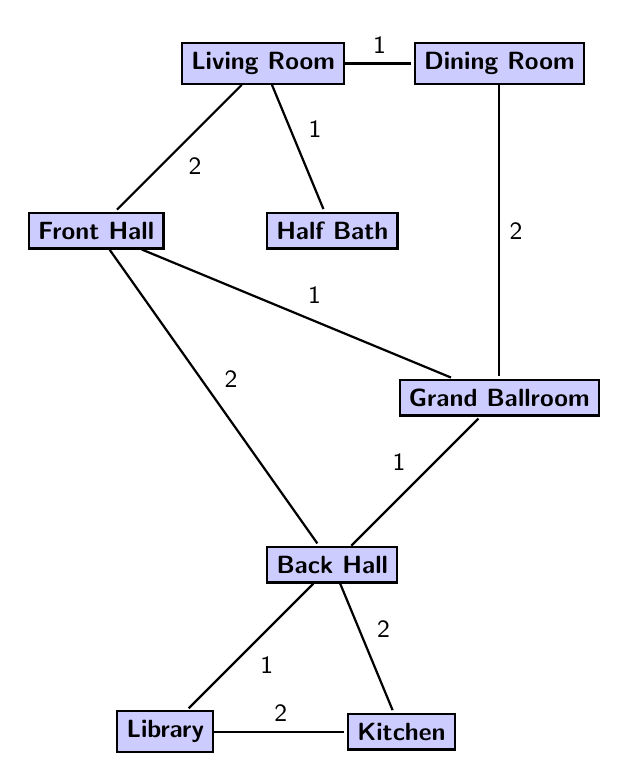
\begin{tikzpicture} [baseline, >=stealth',shorten >=1pt,auto,node distance=3cm,
	thick,main node/.style={rectangle,fill=blue!20,draw,font=\sffamily\small\bfseries}]

	\node[main node] (0) {Living Room};
	\node[main node] (1) [right of=0] {Dining Room};
	\node[main node] (2) [below left of=0] {Front Hall};
	\node[main node] (3) [right of=2] {Half Bath};
	\node[main node] (5) [below right of=3] {Grand Ballroom};
	\node[main node] (4) [below left of=5] {Back Hall};
	\node[main node] (6) [below left of=4]  {Library};
	\node[main node] (7) [right of=6]  {Kitchen};

	\path[every node/.style={font=\sffamily\small}]
	(0) edge node {1} (1)
	(0) edge node {2} (2)
	(0) edge node {1} (3)
	(2) edge node {2} (4)
	(2) edge node {1} (5)
	(1) edge node {2} (5)
	(4) edge node {1} (5)
	(4) edge node {1} (6)
	(4) edge node {2} (7)
	(6) edge node {2} (7);
\end{tikzpicture}

\item For simplicity, I assumed BFS is searching for pre-existing states.\\
	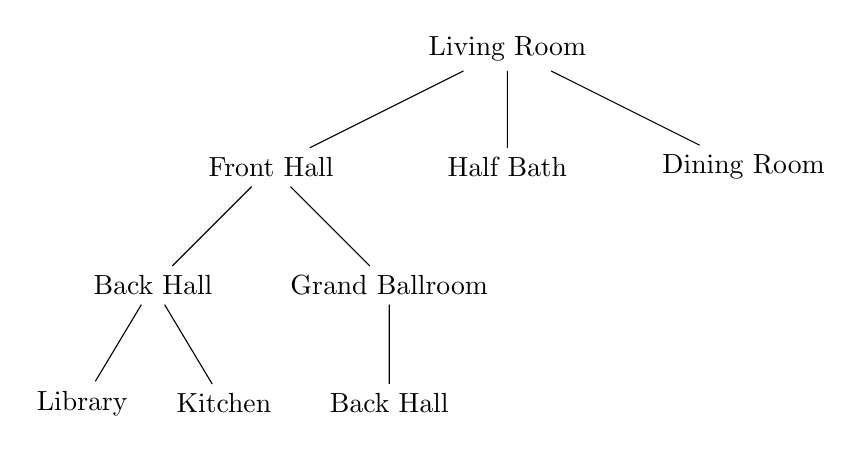
\begin{tikzpicture}[baseline]
	\tikzstyle{level 1}=[sibling distance=30mm] 
	\tikzstyle{level 2}=[sibling distance=30mm] 
	\tikzstyle{level 3}=[sibling distance=18mm] 
	\node{Living Room}
	child{node{Front Hall} child{node{Back Hall} child{node{Library}} child{node{Kitchen}}} child{node{Grand Ballroom} child{node{Back Hall}}}}
	child{node{Half Bath}}
	child{node{Dining Room}};

	\end{tikzpicture}

\item Uniform-cost search: we assume loop detection is used\\
	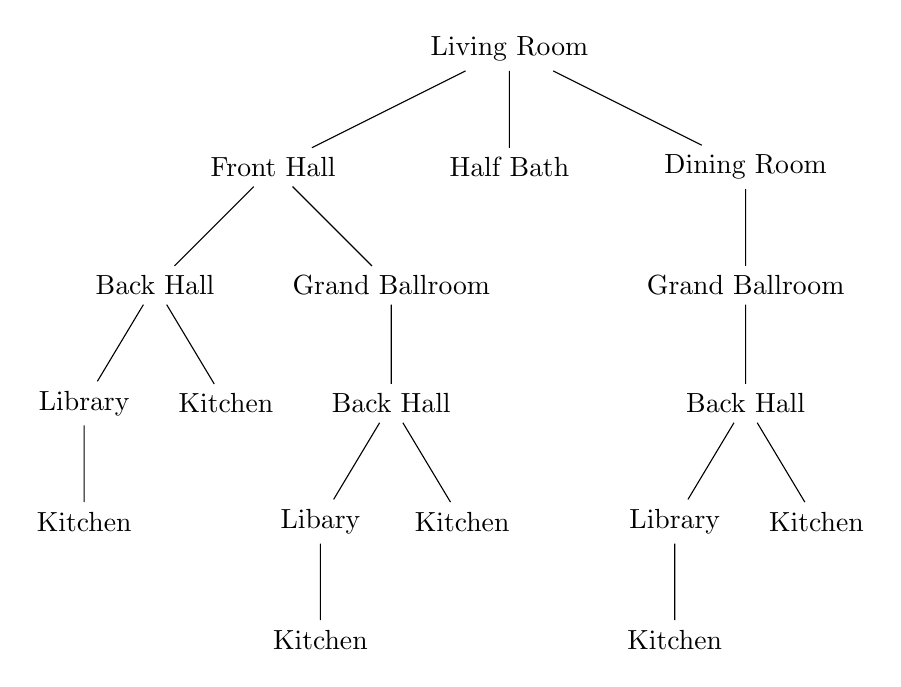
\begin{tikzpicture}[baseline]
	\tikzstyle{level 1}=[sibling distance=30mm] 
	\tikzstyle{level 2}=[sibling distance=30mm] 
	\tikzstyle{level 3}=[sibling distance=18mm] 
	\node{Living Room}
	child{node{Front Hall}
		child{node{Back Hall}
	       child{node{Library}
			   child{node{Kitchen}}}
		   child{node{Kitchen}}}
		child{node{Grand Ballroom}
		   child{node{Back Hall}
	           child{node{Libary}
				  child{node{Kitchen}}}
			   child{node{Kitchen}}}}}
	child{node{Half Bath}}
	child{node{Dining Room} 
		child{node{Grand Ballroom}
		   child{node{Back Hall}
	   		  child{node{Library}
				  child{node{Kitchen}}}
			  child{node{Kitchen}}}}};

	\end{tikzpicture}

\item Depth-first-search:
	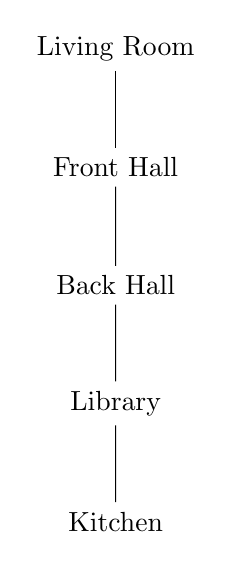
\begin{tikzpicture}[baseline]
	\tikzstyle{level 1}=[sibling distance=30mm] 
	\tikzstyle{level 2}=[sibling distance=30mm] 
	\tikzstyle{level 3}=[sibling distance=18mm] 
	\node{Living Room}
	child{node{Front Hall}
		child{node{Back Hall}
	       child{node{Library}
		      child{node{Kitchen}}}}};
	\end{tikzpicture}

\item Results:\\
	\begin{center} 
		\begin{tabular}{|c|c|c|c| c|c|c|c| c|c|c|c| c|}
			\hline
			& \textbf{BFS:} & nodes & time & cost & \textbf{DFS:} & nodes & time & cost & \textbf{A*:} & nodes & time & cost \\ \hline
			Map 1 &         & 7     & 1ms  & 7    &               & 7     & 2ms  & 7    &              & 7     & 1ms  & 7    \\ \hline
			Map 2 &         & 14    & 1ms  & 7    &               & 14    & 1ms  & 14   &              & 14    & 1ms  & 14   \\ \hline
			Map 3 &         & 31    & 1ms  & 14   &               & 31    & 1ms  & 14   &              & 25    & 1ms  & 14   \\ \hline
			Map 4 &         & 23    & 1ms  & 14   &               & 22    & 1ms  & 18   &              & 24    & 1ms  & 14   \\ \hline
			Map 5 &         & 108   & 2ms  & 15   &               & 29    & 1ms  & 31   &              & 100   & 2ms  & 15   \\ \hline
			Map 6 &         & 979799 & 4.4s & 10090 &             & -     & 21m+  & -     &            & -     & TO & -    \\ \hline
			Map 7 &         & 38    & 2ms  & inf  &               & 46    & 1ms  & inf  &              & 41    & 1ms  & inf  \\ \hline
			Map 8 &         & 22    & 1ms  & 21   &               & 13    & 1ms  & 21   &              & 17    & 1ms  & 15   \\ \hline
	    \end{tabular} 
    \end{center} 

\item I used the A* heuristic of Manhattan distance or L1-norm. This heuristic is admissible because the agent can only move in 4 directions, and therefore needs to make at least the number of moves that Manhatten distance indicates. Therefore, the L1-norm can never be more than than the remaining cost of the solution -- it's optimistic and admissible. 

The main issue is handling map 6. I thought that A* would easily find the way to the goal, but it turns out that it's just not the case. Because the algorithm is optimal and complete, it must consider every cheaper way to get to the goal, which in map 6 means trying out every square in the grid that's closer to the start first. This is what happened with using the L2-norm. Using L1-norm, the case of map 6 is no better than DFS -- the cost of every square is the same, since the heuristic function raises f(n) to be the distance to the goal. But at least we're not first covering every square that's closer to the start point. I think Manhattan distance is as good as we can get since it's the highest we can push h(n) while still being admissible.

\item DFS is great in problems where you know the maximum depth the problem can go to. A classic example of this is the N queens problem. BFS attempts to map out the whole space one depth level at a time, which with a large N becomes intractable. DFS doesn't use nearly as much memory (in general), and in particular in this case, goes down only N levels.

\item DFS's big deficiency is that it lacks the full view (up to a certain depth) of the whole state-space that is very helpful for BFS in some scenarios. BFS is stronger in a problem where the branching factor is relatively low but the depth is very deep and where BFS's liberal usage of memory allows it to recognize previously visited states and eliminate them. A prime example is map6, where the branching factor is only 4, and many paths visit the same states over and over again. BFS is able to recognize previously visited states and skip them in the next visits, making it the most efficient algorithm for handling map6. DFS, by constrast, keeps only enough information to prevent loops, and therefore wastes a lot of time expanding the same states over and over again.

\item A* is limited by its admissibility constraint, which prevents the heuristic from dominating the cost-based expansion of $g(n)$. This allows A* to remain optimal, but it also means every path must be investigated, but without the advanced repeat state avoidance of BFS. In a case where A* is presented with nodes of very different cost, A* does quite well and is able to choose a cheaper path than BFS. A worst-case scenario happens in something like map 6, where every node is uniform cost. Even though the heuristic $h(n)$ indicates the right direction in which to go, the admissibility constraint means that A* has to investigate every low-cost uniform path.

\item \begin{enumerate}
	  \item Euclidean distance is admissible and it is fairly useful. However, it does little to offset the cost function $g(n)$ -- it doesn't come close enough to the true cost.
	  \item Twice the Euclidean distance is not admissible, as can be seen by a simple example where the start point and the goal point are on a straight line. $h(n)$ will be twice the distance to the goal, which is more than the minimal cost to the goal can be.

      \item Manhattan distance is what I found to be closest to the true cost of the problem, and therefore the best heuristic. In the worst case, the path from start to the goal is exactly equivalent to the Manhattan distance and every step has the same cost. In this case, A* doesn't know which way to go (every step has the same cost) but at least it's not busy searching BFS-style. At best, A* can avoid expensive obstacles along the way and get to the goal much more cheaply than BFS and DFS.

	  \item Twice the Manhattan distance is not admissible, for the same reason as discussed earlier regarding twice the Euclidean distance.

	  \item By setting h(n) to 2 for all n, the effect is the same as cancelling the $h(n)$ factor and making $f(n) = g(n)$. This is the same as uniform cost search. It also is inadmissible for certain trivial problems where the goal is less than 2 steps away from the start position.

	  \item 0 if $n$ is the goal, 1 otherwise, is admissible, since the goal is at least one step away from the start position. It cancels out the $h(n)$ factor though, much as the previous question did. $f(n)$ is therefore equivalent to $g(n)$.
	  \end{enumerate}

\item For long distance flights, the shape of the Earth becomes a factor when planning the flightpath. Since the Earth is nearly spherical, the shortest distance between two points no longer obeys Euclidean gemometry, and orthodromic distance is needed instead. Since the best path between 2 points it less than what Euclidean distance predicts, h(n) is larger than the potential minimal cost of the problem and therefore is not admissible. Orthodromic or great-circle distance is used instead.

\end{enumerate}

\end{document}

